\newpage
\section*{Pregunta 3}
Describe las principales características de los distintos paradigmas
de programación (Estructurado, Orientado a Objetos, Funcional y Lógico)
y da a 2 ejemplos de lenguajes de programación de cada paradigma.

$\rhd$ Para esta pregunta, explicamos cada parádigma por separado,
esto es
\begin{center}
  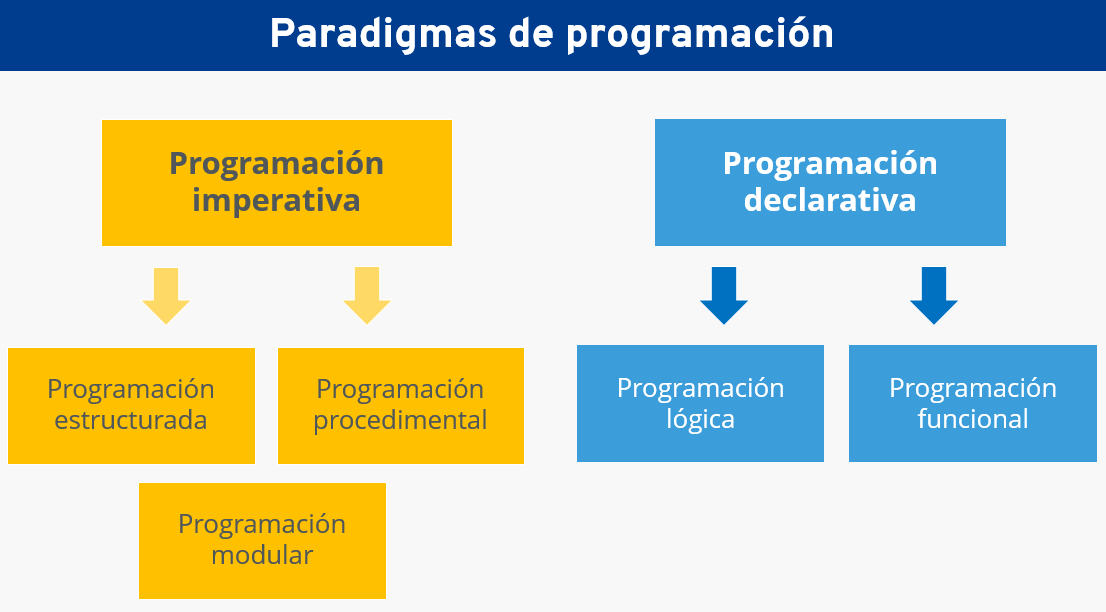
\includegraphics[scale=0.40]{./Paradigmas.png}
\end{center}

\subsection*{Parádigma Imperativo}
Describe la programación en términos del estado del programa
y sentecnias que cambian dicho estado. Se le debe explicar
el como hacer las cosas.

\begin{itemize}
\item \textbf{Orientado a objetos.}
Las principales características en las orientación a objetos
son; el polimorfismo (diseñar objetos que compartan comportamientos,
y los puedan heredar), encapsulamiento (la información referente
a un objeto esta contenida en este y puede no ser accesible al
exterior), reutilización de código (modularizar nos permite evitar
duplicar código), los conceptos de clases y objetos (nuestros
objetos tendrán comportamientos definidos en clases).

Ejemplos de lenguajes orientados a objetos:
\begin{enumerate}
\item C++.
\item JAVA.
\end{enumerate}
\item \textbf{Estructurado.}
Las principales características en los lenguajes estructurados
son; la sintaxis (orden y reglas del lenguaje), la semántica
(interpretación y significado de la sintaxis), la pragmática
(modo en que el contexto o situación le entrega interpretación
al significado).

Ejemplos de lenguajes estructurados:
\begin{enumerate}
\item C.
\item PASCAL.
\end{enumerate}
\end{itemize}
\subsection*{Parádigma Declarativo}
Este paradigma de programación esta basado en el desarrollo de
programas ``declarando'' un conjunto de condiciones, proposiciones,
afirmaciones, restricciones, ecuaciones o transformaciones que
describen el que requiera y no el como hacer.

\begin{itemize}
\item \textbf{Funcional.}
Las principales características de la programación funcional
son; semántica limpia (no hay ambigüedades en el significado
de las funciones, almacenamiento implícito de datos),
inexistencia de efectos colaterales (no hay asignación a
variables globales), utilización del cálculo-$\lambda$ (independencia
fuera de la función).

Ejemplos de lenguajes funcionales:
\begin{enumerate}
\item Racket.
\item Haskell.
\end{enumerate}
\item \textbf{Lógico.}
Las principales características de los lenguajes en el paradigma lógico
son; reglas (conjunto de proposiciones lógicas escritas como clausulas
de Horn), hechos (Expresiones atómicas que verifican un predicado sobre
algunos entes que puede procesar el mismo), consultas (proposiciones
que se verifican para algún valor de verdad), recursión.

Ejemplos de lenguajes lógicos:
\begin{enumerate}
\item GODEL.
\item PROLOG.
\end{enumerate}
\end{itemize}
\hfill $\lhd$
